\begin{itemize}

\item Trong quá trình xây dựng mô hình miền, cần có trao đổi giữa người thiết kế hệ thống và chuyên gia ngành để hiểu đúng về miền. Tuy nhiên, nhóm kinh doanh sử dụng ngôn ngữ kinh doanh và nhóm công nghệ có xu hướng sử dụng các thuật ngữ kỹ thuật trong giao tiếp của họ. Người phát triển phần mềm tập trung vào lớp, phương thức, thuật toán, trong khi chuyên gia ngành thường sử dụng ngôn ngữ chuyên ngành của họ. Sự khác biệt về ngôn ngữ giữa các thành viên có thể dẫn đến những thách thức về giao tiếp.

\item Ngoài ra, trong các lĩnh vực kinh doanh khác nhau, một thuật ngữ có thể được sử dụng trong nhiều miền, cùng với ý nghĩa khác nhau gây ra sự nhầm lẫn và hiểu sai cho các người phát triển phần mềm cũng như các chuyên gia ngành.

$\Rightarrow$ Thiết kế hướng miền đề xuất sử dụng ngôn ngữ chung để giải quyết những thách thức ngôn ngữ.

\item Ngôn ngữ chung (Ubiquitous Language) là một ngôn ngữ được cấu trúc xung quanh mô hình miền và được tất cả các thành viên trong nhóm sử dụng cho mọi hoạt động của nhóm với phần mềm.

\item Ngôn ngữ chung được xác định bởi các từ vựng và có định nghĩa rõ ràng về ngữ cảnh sử dụng từ vựng.

\end{itemize}

\subsubsection{Một số đặc điểm của ngôn ngữ chung}

\begin{itemize}

\item Ngôn ngữ chung được sử dụng bởi cả chuyên gia ngành và chuyên gia công nghệ.

\item Có nhiều ngôn ngữ chung trong một tổ chức được mỗi nhóm tạo và quản lý một cách độc lập.

\item Việc tạo ra ngôn ngữ chung là một quá trình liên tục.

Ngôn ngữ chung phát triển theo thời gian thông qua sự cộng tác giữa doanh nghiệp và các chuyên gia công nghệ.

\item Các thành viên phải sử dụng ngôn ngữ chung cho công việc và trong toàn bộ hệ thống:

\begin{itemize}

\item Các chuyên gia ngành sử dụng.

\item Các chuyên gia công nghệ sử dụng.

\item Sử dụng trong cuộc thảo luận trao đổi.

\item Sử dụng trong các tài liệu phát triển.

\item Sử dụng trong sản phẩm phần mềm.

\item Sử dụng trong kiểm thử phần mềm.

\end{itemize}

\end{itemize}

\begin{figure}[H]

\centering

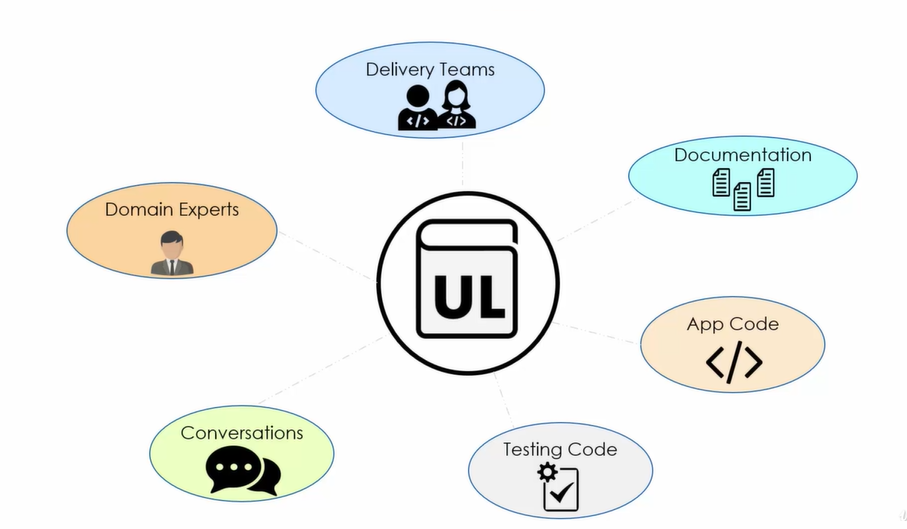
\includegraphics[scale = 0.6]{pictures/ngon_ngu_chung/main.png}

\caption{Ngôn ngữ chung được sử dụng trong toàn bộ hệ thống}

\end{figure}

%!<! - - Hướng dẫn 5/7 - - >

